% !TeX root = ../thuthesis-example.tex

\begin{translation}
\label{cha:translation}

\title{基于深度残差U-Net网络的道路提取}
\maketitle

\tableofcontents

\section{摘要}

航空影像道路提取⼀直是遥感影像分析领域的研究热点。本文提出了一种将残差学习和U-Net优势相结合的语义分割神经网络,用于道路区域提取。该网络由残差块构建,具有与U-Net相似的架构。该模型主要有两个优势:首先,残差块简化了深度网络的训练。其次,网络中丰富的跳跃连接可以促进信息传播,使我们能够设计具有更少参数但性能更好的网络。我们在一个公共道路数据集上测试了我们的网络,并将其与U-Net和其他两种最先进的基于深度学习的道路提取方法进行比较。所提出的方法与其他方法相比展现出了很大优势,证明了其相对近期其他最新技术的优越性。

\textbf{关键词:}道路提取;卷积神经网络;深度残差U-Net

\section{引言}

道路提取是遥感领域的基本任务之一。它有着广泛的应用,如自动道路导航、无人驾驶车辆、城市规划和地理信息更新等。虽然在过去十年中受到了广泛关注,但由于原始遥感图像中的噪声、遮挡和背景的复杂性,从高分辨率遥感图像中提取道路仍然是一项具有挑战性的任务。

近年来,人们提出了多种从遥感图像中提取道路的方法。这些方法主要分为两类:道路区域提取和道路中心线提取。道路区域提取\cite{1,2,3,4,5,6}可以生成道路的像素级标签,而道路中心线提取\cite{7,8}旨在检测道路骨架。还有一些方法可以同时提取道路区域和中心线\cite{9}。由于使用形态学细化等算法可以很容易地从道路区域获得道路中心线\cite{10},故本文侧重于从高分辨率遥感图像中提取道路区域。

道路区域提取可以看作是一个分割或像素级分类问题。例如,Song和Civco\cite{11}提出了一种利用形状指数特征和支持向量机(SVM)检测道路区域的方法。Das等人\cite{12}利用道路的两个显著特征,设计了一个多级框架,使用概率SVM从高分辨率多光谱图像中提取道路。Alshehhi和Marpu\cite{6}提出了一种基于层次图的图像分割的无监督道路提取方法。

近年来,深度学习取得了巨大进展。基于深度神经网络的方法在各种计算机视觉任务上取得了最先进的性能,如场景识别\cite{13}和目标检测\cite{14}。遥感界的研究人员还试图利用深层神经网络来解决遥感数据的解释和理解问题\cite{2,3,4,5}\cite{15,16,17,18}。这些方法提供了比传统方法更好的结果,显示了应用深度学习技术分析遥感任务的巨大潜力。

Mnih和Hinton首次在道路提取领域尝试应用深度学习技术\cite{2}。他们提出了一种利用受限玻耳兹曼机(RBM)从高分辨率航空图像中检测道路区域的方法。为了获得更好的结果,他们应用了检测前的预处理和检测后的后处理。进行了预处理的目的是降低输入数据的维数。而采用后处理是来清除断开斑点并填充道路中的孔洞。与Mnih和Hinton的方法\cite{2}不同,Saito等人\cite{5}采用卷积神经网络(CNN)直接从原始遥感图像中提取建筑物和道路,该方法使用RBM作为构建深层神经网络的基本块。在马萨诸塞州道路数据集上,该方法比Mnih和Hinton的方法\cite{2}取得了更好的结果。

最近,许多研究表明,更深的网络会有更好的性能\cite{19,20}。然而,由于梯度消失等问题,很难训练非常深的体系结构。为了克服这个问题,何凯明等人\cite{21}提出了深度残差网络,利用恒等映射来促进训练。Ronneberger等人\cite{24}提出了将不同层次的特征映射串联起来的U-Net,而不是在完全卷积网络(FCN)\cite{23}中使用跳跃连接,以提高分割精确率。U-Net结合了低级细节信息和高级语义信息,因此在生物医学图像分割方面取得了很好的性能\cite{24}。

受深度残差网络\cite{21}和U-Net\cite{24}的启发,本文中,我们提出了深度残差U-Net(ResUnet),这是一种利用深度残差学习和U-Net体系结构优势的体系结构。所提出的(ResUnet)是基于U-Net的体系结构构建的。我们的ResUnet和U-Net之间的差异有两个方面。首先,我们使用残差块代替普通神经单元作为基本块来构建深度网络。其次,裁剪操作是不必要的,因此我们在我们的网络中删除了裁剪操作,从而获得了更精妙的结构和更好的性能。

\section{方法}
\subsection{深度ResUnet}
\subsubsection{U-Net}
在语义分割中,为了获得更好的结果,在保留高级语义信息的同时使用低级细节是非常重要的\cite{23,24}。然而,训练这样一个深层次的神经网络非常困难,尤其是当只有有限的训练样本可用时。解决此问题的一种方法是使用预先训练好的网络,然后在目标数据集上对其进行微调,如\cite{23}中所述。另一种方法是采用广泛的数据扩充,如U-Net中所做的那样\cite{24}。除了数据扩充之外,我们相信U-Net的结构也有助于缓解训练问题。这背后的直觉是,将低级特征复制到相应的高级实际上创建了一条信息传播路径,允许信号以更容易的方式在低级和高级之间传播,这不仅有助于在训练期间反向传播,而且还可以将低级更细的细节补偿到高级语义特征。这在某种程度上与残差神经网络的想法相似\cite{21}。本文中,我们证明,通过用残差块替换普通单元,可以进一步提高U-Net的性能。
\begin{figure}[t!]
	\begin{center}
		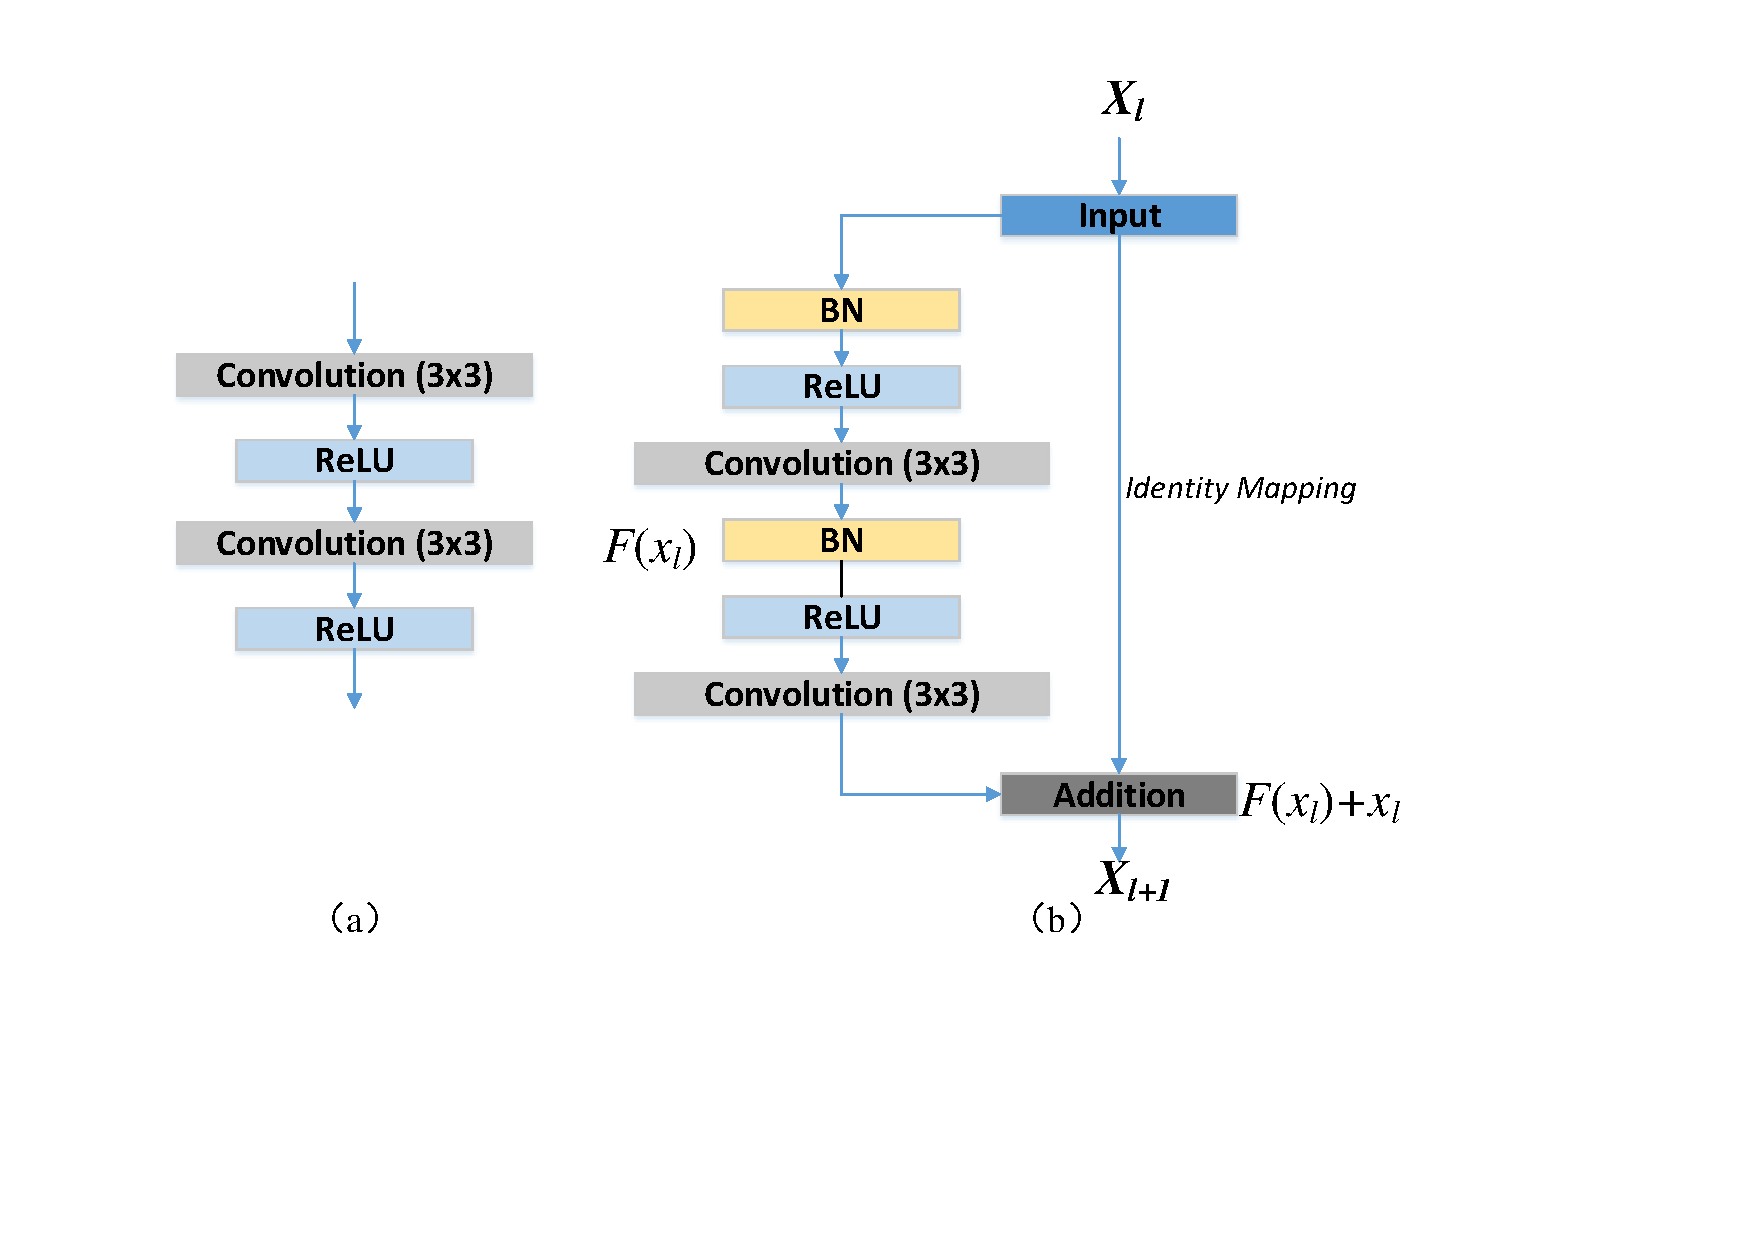
\includegraphics[width=0.6\columnwidth]{res-u-net-blocks.pdf}
		\caption{神经网络的构建模块。(a) U-Net中使用的普通神经单元和(b)本文提出的的ResUnet中使用的具有恒等映射的残差块。}
		\label{Fig:ResNet Block}
	\end{center}
\end{figure}
\subsubsection{残差块}
深入将改善多层神经网络的性能,但可能会妨碍训练,并可能出现退化问题\cite{21}。为了克服这些问题,He等人\cite{21}提出了残差神经网络,以便于训练和解决退化问题。残差神经网络由一系列叠加的残差块组成。每个残差块可表示为一般形式:
\begin{equation}\label{Equ:Residual Uint}
  \begin{split}
  \mathbf{y}_{l}\ \ \ & = h(\mathbf{x}_{l})+\mathcal{F}(\mathbf{x}_{l}, \mathcal{W}_{l}), \\
  \mathbf{x}_{l+1} & = f(\mathbf{y}_{l}),
  \end{split}
\end{equation}
其中$\mathbf{x}_{l}$和$\mathbf{x}_{l+1}$是第$l$个残差块,$\mathcal{F}(\cdot)$是残差函数, $f(\mathbf{y}_l)$是激活函数,$h(\mathbf{x}_{l})$是恒等映射,例如$h(\mathbf{x}_{l}) = \mathbf{x}_{l}$这样的。图~\ref{Fig:ResNet Block}显示了普通单元和残差块之间的差异。在一个残差块中存在批量归一化(BN)、ReLU激活和卷积层的多种组合。He等人\cite{22}详细讨论了不同组合的影响,并提出了完整的预激活设计,如图~\ref{Fig:ResNet Block}(b)所示。在这项工作中,我们还使用全预激活残差块来构建我们的深度残差U-Net网络。
\begin{figure}[tbp!]
	\begin{center}
		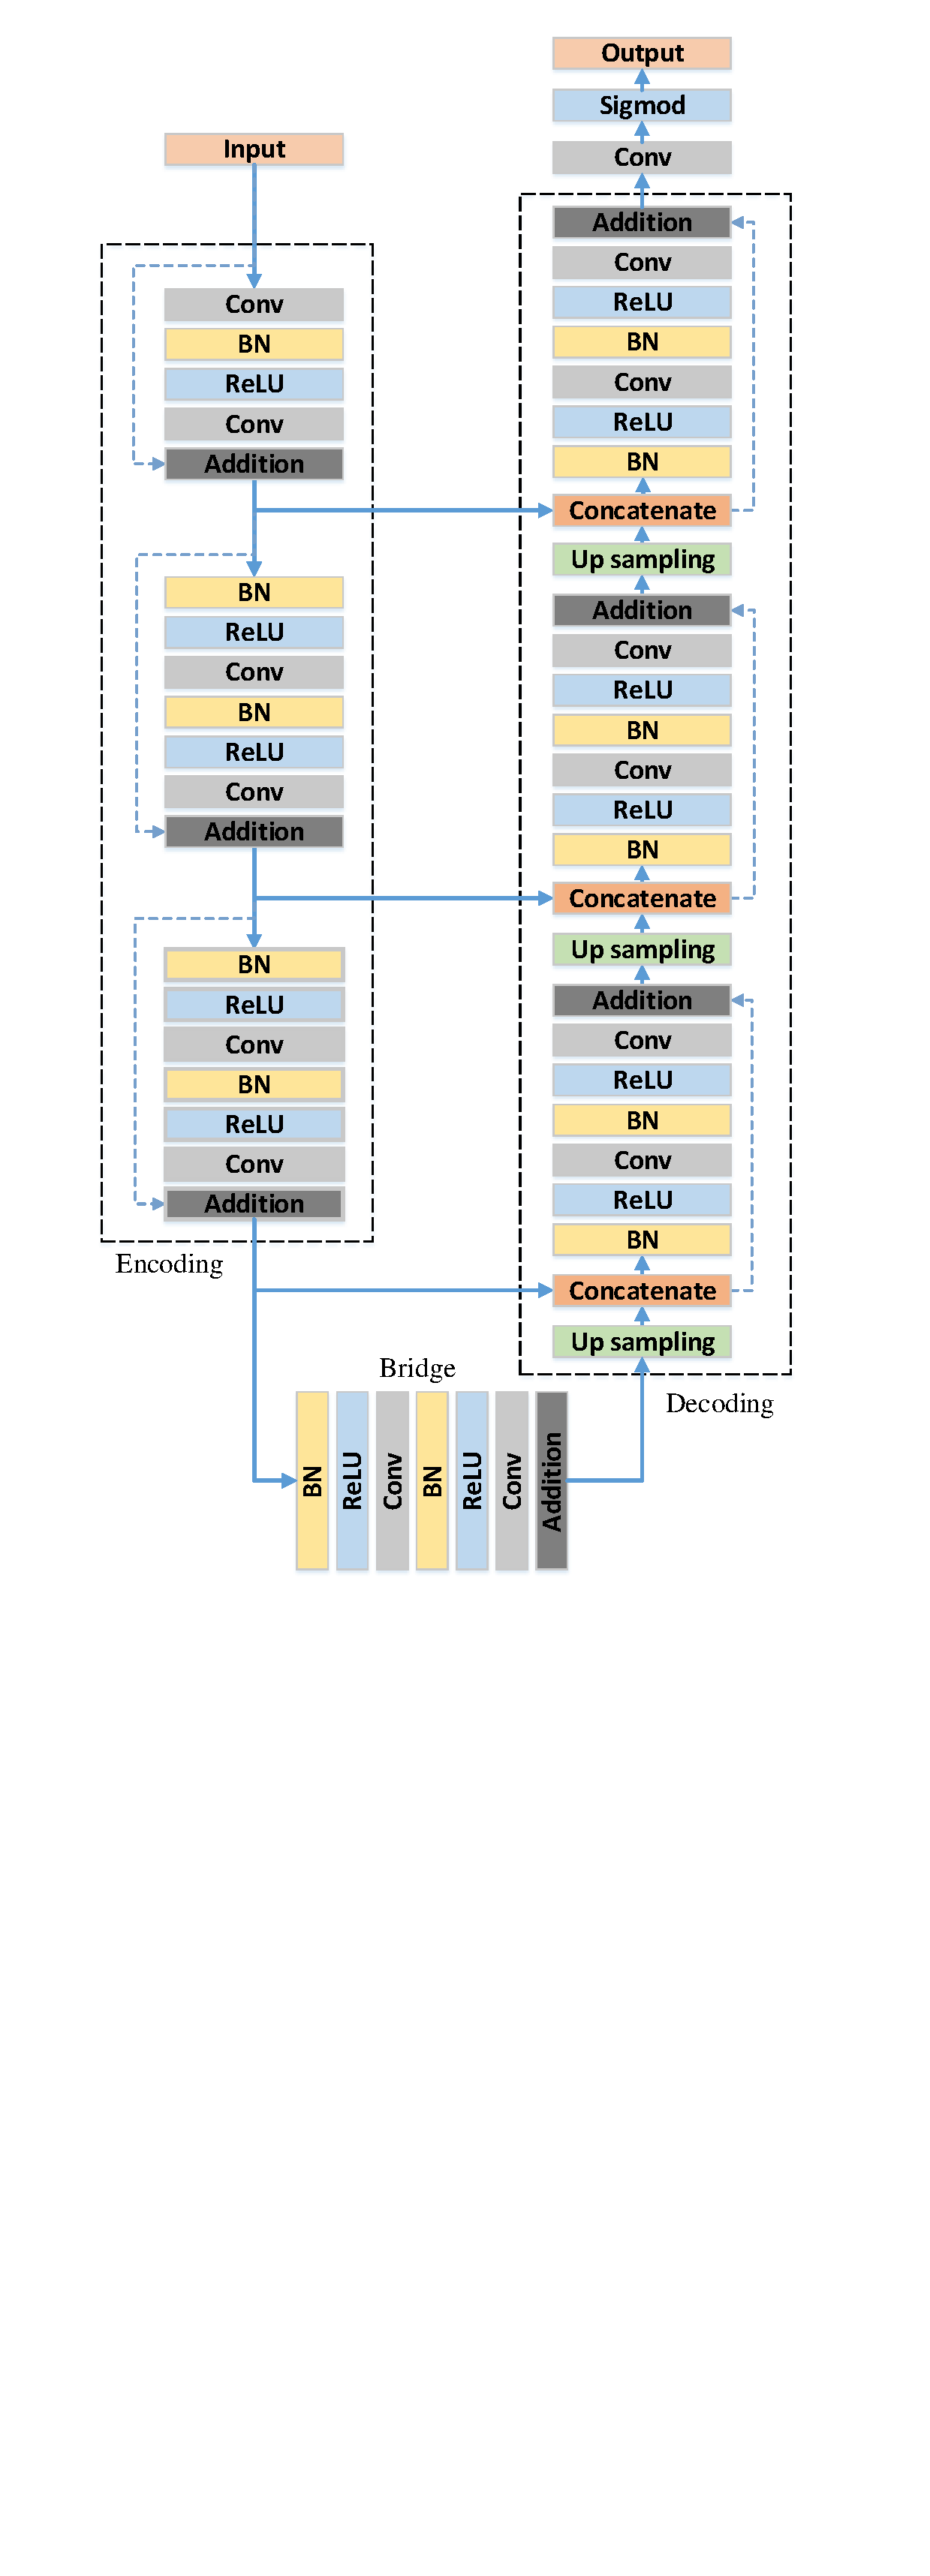
\includegraphics[width=0.6\columnwidth]{ResUNet.pdf}
		\caption{本文提出的ResUnet网络结构}
		\label{Fig:Deep Res-U-Net}
	\end{center}
\end{figure}

\subsubsection{Deep ResUnet}
在这里,我们提出了deep ResUnet,这是一种结合了U-Net和残差神经网络优点的语义分割神经网络。这种组合给我们带来了两个好处:1)残差块将简化网络训练;2)残差块内以及网络低层和高层之间的跳跃连接将促进信息传播而不会退化,从而可以设计参数更少的神经网络,但可以在语义分割方面取得更好的性能。

在这项工作中,我们使用deep ResUnet的7级体系结构进行道路区域提取,如图~\ref{Fig:Deep Res-U-Net}所示。该网络由编码、桥接和反编码三部分组成。\footnote{U-Net使用“收缩”和“扩展”路径来表示网络的特征提取和上卷积阶段。在本文中,我们更喜欢术语编码和解码,因为我们认为它更有意义,更容易理解}第一部分将输入图像编码为紧凑的表示形式。最后一部分将表示恢复为像素级分类,即语义分割。中间部分就像连接编码和解码路径的桥梁。这三个部分都是用残差块构建的,残差块由两个$3\times 3$卷积块和一个单位映射组成。每个卷积块包括BN层、ReLU激活层和卷积层。标识映射连接单元的输入和输出。

编码路径有三个残差块。在每个单元中,不是使用池操作来减小特征映射大小的采样,而是对第一个卷积块执行步长为2的卷积操作,以将特征映射减少一半。相应地,解码路径也由三个残差块组成。在每个单元之前,从较低级别对特征映射进行上采样,并与相应编码路径中的特征映射进行串联。在最后一级解码路径之后,使用$1\times1$卷积和sigmod激活层将多通道特征映射投影到所需的分割中。我们总共有15个卷积层,而U-Net有23个卷积层。值得注意的是,U-Net中不可或缺的裁剪在我们的网络中是不必要的。每个步骤的参数和输出大小如表~\ref{Table:Feature Size}所示。
\begin{table}[!htb]
	\tiny
	\centering
	\caption{ResUnet的网络结构}	
	\label{Table:Feature Size}	
	\begin{tabular}{ccllcl}
		\hline
		\hline
		& Unit level  & Conv layer & Filter  & Stride &  Output size\\
		\hline
		Input                      &        &     &   &    &  $224\times 224 \times 3$ \\
		\hline	
		\multirow{6}{*}{Encoding}
		& \multirow{2}{*}{Level 1}& Conv 1  & $3\times 3/64$ & 1 &  $224\times 224 \times 64$ \\
		&        & Conv 2  &  $3\times 3/64$ & 1 &  $224\times 224 \times 64$ \\
		\cline{2-6}			
		& \multirow{2}{*}{Level 2}& Conv 3  &  $3\times 3/128$ & 2 &  $112\times 112 \times 128$ \\
		&        & Conv 4  &  $3\times 3/128$ & 1 &  $112\times 112 \times 128$ \\
		\cline{2-6}
		& \multirow{2}{*}{Level 3}& Conv 5  &  $3\times 3/256$ & 2 &  $56\times 56 \times 256$ \\
		&        & Conv 6  &  $3\times 3/256$ & 1 &  $56\times 56 \times 256$ \\
		\cline{2-6}						
		\hline
		\multirow{2}{*}{Bridge}
		&\multirow{2}{*}{Level 4}         &Conv 7  &  $3\times 3/512$ & 2 &  $28\times 28 \times 512$ \\
		&	      &Conv 8 &  $3\times 3/512$ & 1 &  $28\times 28 \times 512$\\
		\hline
		\multirow{6}{*}{Decoding}	
		& \multirow{2}{*}{Level 5} &Conv 9 &  $3\times 3/256$ & 1 &  $56\times 56 \times 256$ \\
		&        &Conv 10 &  $3\times 3/256$ & 1 & $56\times 56 \times 256$ \\
		\cline{2-6}
		& \multirow{2}{*}{Level 6} &Conv 11 &  $3\times 3/128$ & 1 &  $112\times 112 \times 128$ \\
		&        &Conv 12 &  $3\times 3/128$ & 1 &  $112\times 112 \times 128$ \\
		\cline{2-6}			
		& \multirow{2}{*}{Level 7} &Conv 13 &  $3\times 3/64$ & 1 &   $224\times 224 \times 64$ \\
		&        &Conv 14 &  $3\times 3/64$ & 1 &  $224\times 224 \times 64$ \\
		\hline
		Output                      &        &Conv 15 &  $1\times 1$ & 1 &  $224\times 224 \times 1$ \\		
		\hline
		\hline
	\end{tabular}
\end{table}

\subsection{损失函数}

给定一组训练图像和相应的地面真值分割$\{I_i,s_i\}$,我们的目标是估计网络的参数$W$,以便生成准确而稳健的道路区域。这是通过最大限度地减少由$Net(I_i;W)$和地面真相$s_i$生成的分段之间的损失来实现的。在本文中,我们使用均方误差(MSE)作为损失函数:
\begin{equation}\label{Equ:mse}
  \mathcal{L}(W) = \frac{1}{N}\sum\limits^{N}_{i=1}||Net(I_i;W) - s_i||^2,
\end{equation}
其中$N$是训练样本数。我们使用随机梯度下降(SGD)来训练我们的网络。众所周知,其他可推导的损耗函数也可用于训练网络。例如,U-Net采用像素交叉熵作为损失函数来优化模型。

\subsection{结果优化}

我们的语义切分网络的输入和输出在宽度和高度上都是相同的,即$224\times224$。由于卷积层中的零填充,输出边界附近的像素精确率会低于中心像素。为了得到更好的分割结果,我们使用了重叠策略来生成大图像的分割结果。输入子图像是从原始图像中裁剪出来的,重叠度为$o$(在我们的实验中$o=14$)。最后的结果是通过将所有子分割拼接在一起得到的。重叠区域中的值会取平均值。

\section{实验}

为了证明所提出的deep ResUnet的准确性和效率,我们在马萨诸塞州道路数据集\footnote{https://www.cs.toronto.edu/\~{}vmnih/data/}上对其进行了测试,并将其与Mnih的~\cite{2}方法、Saito~\cite{5}的方法和U-Net~\cite{24}这三种最新方法作了比较。

\subsection{数据集}

马萨诸塞州道路数据集由Mihn等人建立~\cite{2}。该数据集共包含1171幅图像,其中1108幅用于训练,14幅用于验证,49幅用于测试。此数据集中所有图像的大小为$1500\times1500$像素,分辨率为1.2米/像素。该数据集大致涵盖了从城市、次城市到农村地区的500 km$^2$的空间交叉以及广泛的地物,包括道路、河流、海洋、各种建筑物、植被、学校、桥梁、港口、车辆等。在本文中,我们在该数据集的训练集上训练我们的网络,并在其测试集上报告结果。

\subsection{实现细节}

该模型采用Keras\cite{25}框架实现,并通过SGD算法最小化损失函数.~\ref{Equ:mse}进行优化。有1108张大小为$1500\times1500$的训练图像可用于训练。理论上,我们的网络可以将任意大小的图像作为输入,但是需要大量的GPU内存来存储特征地图。在本文中,我们使用固定大小的训练图像($224\times224$,如表~\ref{Table:Feature Size})来训练模型。这些训练图像是从原始图像中随机抽取的。最后,生成30000个样本并反馈到网络中学习参数。应注意的是,训练期间未使用数据扩充。我们开始在NVIDIA Titan 1080 GPU上以8个小批量训练模型。最初,学习率设置为0.001,每20个周期(epoch)衰减为0.1倍。网络将在50个周期(epoch)内收敛。

\subsection{评价指标}

评估二进制分类方法最常用的指标是精确率和召回率。在遥感中,这些指标也称为正确度和完整度。精确率是预测为道路像素的比率,召回率是正确预测为道路像素的比率。

由于很难正确标记所有道路像素,Mnih等人\cite{2}在道路提取中引入了宽松的精确率和召回率\cite{26}。松弛精确率定义为$\rho$像素范围内预测为道路的像素数与标记为道路的像素数的比率。松弛召回率是标记为道路的像素数与预测为道路的像素数之间$\rho$像素范围内的比率。在本实验中,松弛参数$\rho$设置为3,这与之前的研究\cite{2,5}一致。我们还报告了不同方法的盈亏平衡点。盈亏平衡点定义为松弛精度召回曲线上的点,其精确率值等于召回率。换句话说,盈亏平衡点是松弛精度召回曲线和线y=x的交点。

\subsection{对比研究}

在马萨诸塞州道路数据集的测试集上,我们比较了三种基于深度学习的道路提取方法。表~\ref{Table:Value at Breakeven Point}展示了本文方法和所对比方法的盈亏平衡点。图~\ref{Fig:PR}显示了U-Net和我们的网络的松弛精确率召回曲线及其盈亏平衡点,以及所比较方法的盈亏平衡点。可以看出,我们的方法在松弛精确率和召回率方面优于所有其他三种方法。虽然我们的网络参数仅为U-Net的$1/4$(7.8M vs 30.6M),但在道路提取任务上取得了有希望的改进。

\begin{table}[!hbp]
  \begin{center}
  \caption{在马萨诸塞州道路数据集上,就盈亏平衡点对提出的和其他三种基于深度学习的道路提取方法进行了比较。盈亏平衡点越高,表示在精确率和召回率方面的性能越好。}
  \label{Table:Value at Breakeven Point}
  \begin{tabular}{l|c}
  \hline
  Model & Breakeven point\\
  \hline
  Mnih-CNN\cite{2} & 0.8873  \\
  \hline
  Mnih-CNN+CRF\cite{2} & 0.8904  \\
  \hline
  Mnih-CNN+Post-Processing\cite{2} & 0.9006  \\
  \hline
  Saito-CNN\cite{5} & 0.9047 \\
  \hline
  U-Net\cite{24} & 0.9053 \\
  \hline
  ResUnet & \textbf{0.9187} \\
  \hline
  \end{tabular}
  \end{center}
\end{table}

\begin{figure}[!t]
  \begin{center}
      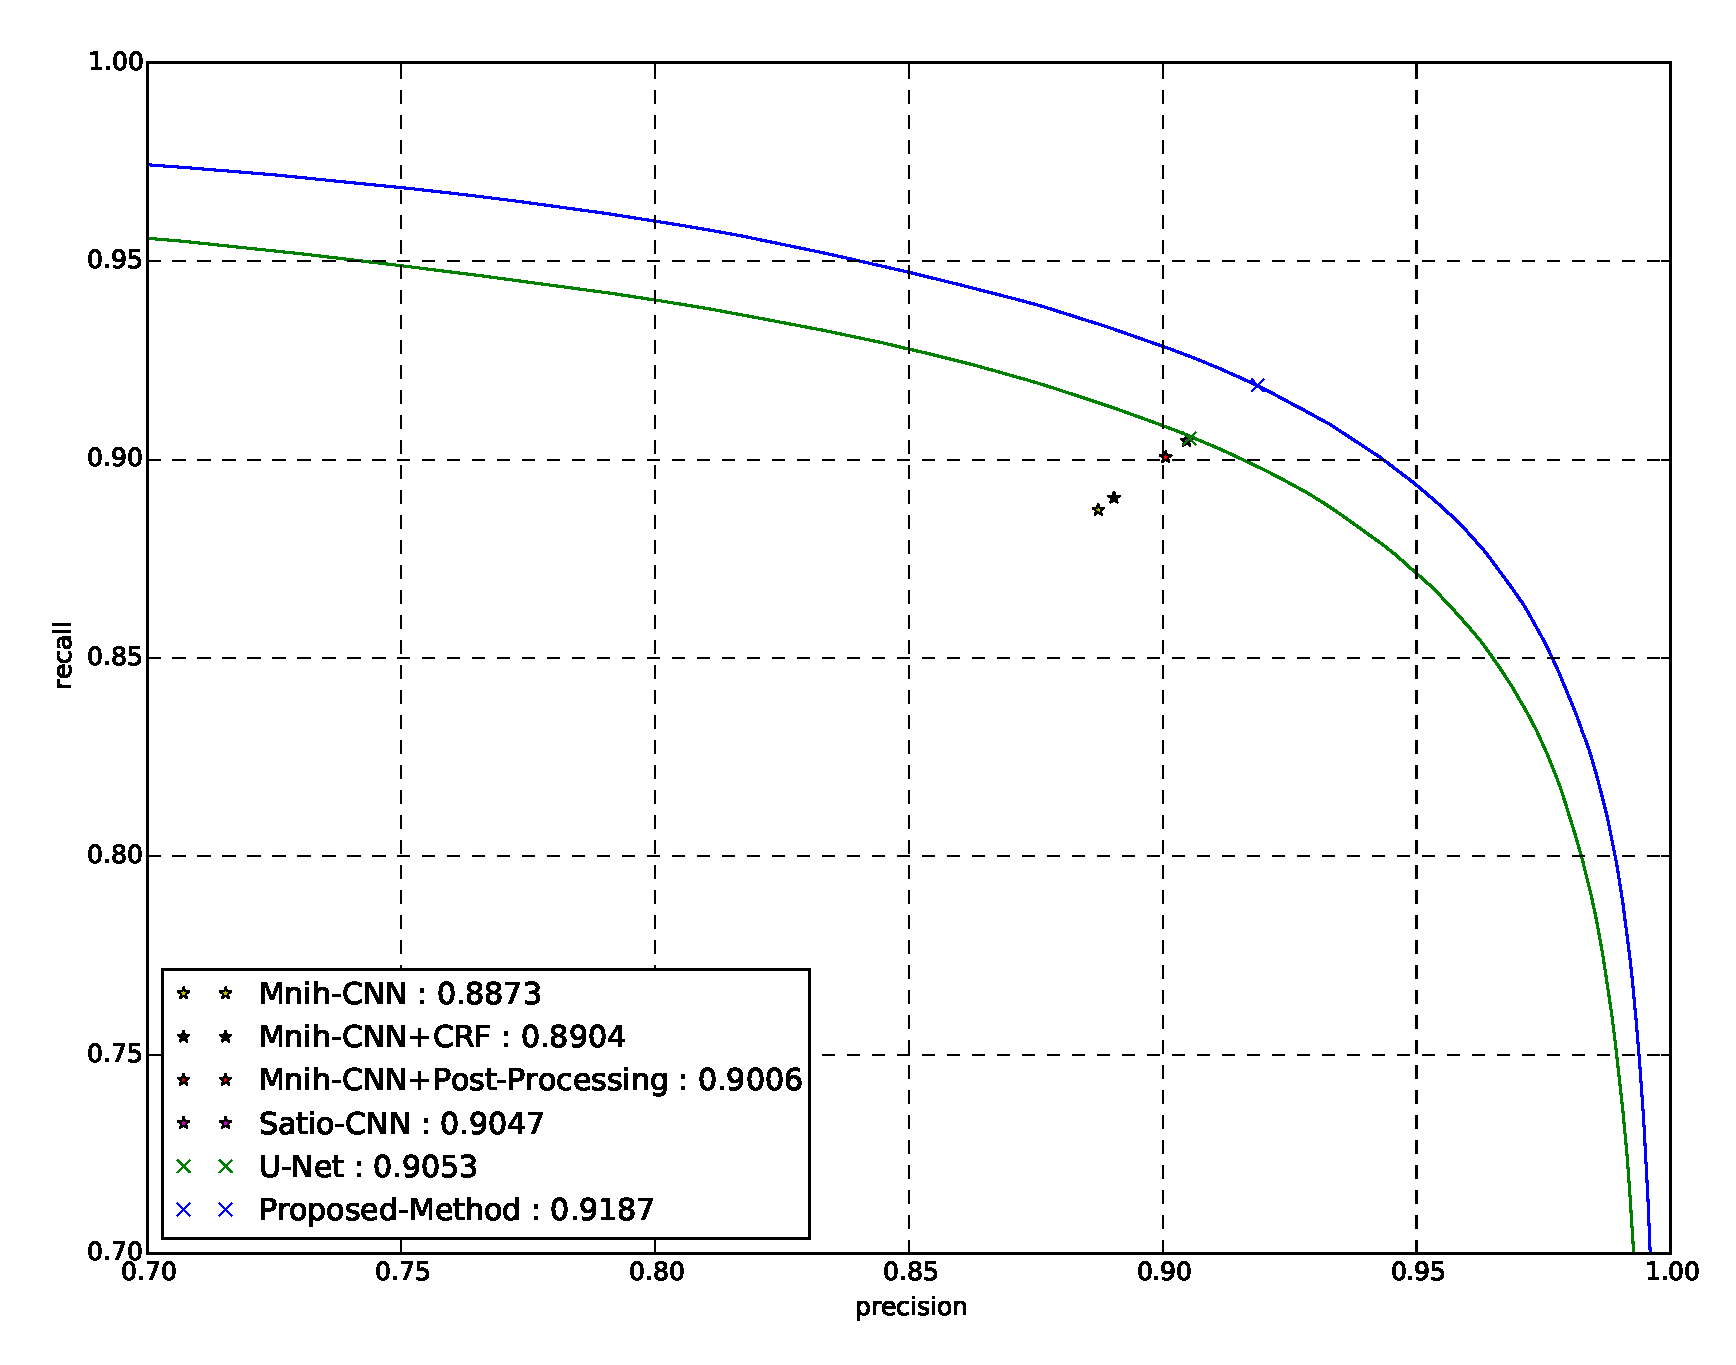
\includegraphics[width=1\columnwidth]{pr1.pdf}
        \caption{U-Net和本文提出的方法的松弛精度召回曲线在马萨诸塞州道路数据集上的对比。标记“$\star$”和“$\times$”的是不同方法的盈亏平衡点。}
        \label{Fig:PR}
  \end{center}
  \end{figure}
  
  \begin{figure*}[ht]
  \begin{center}
      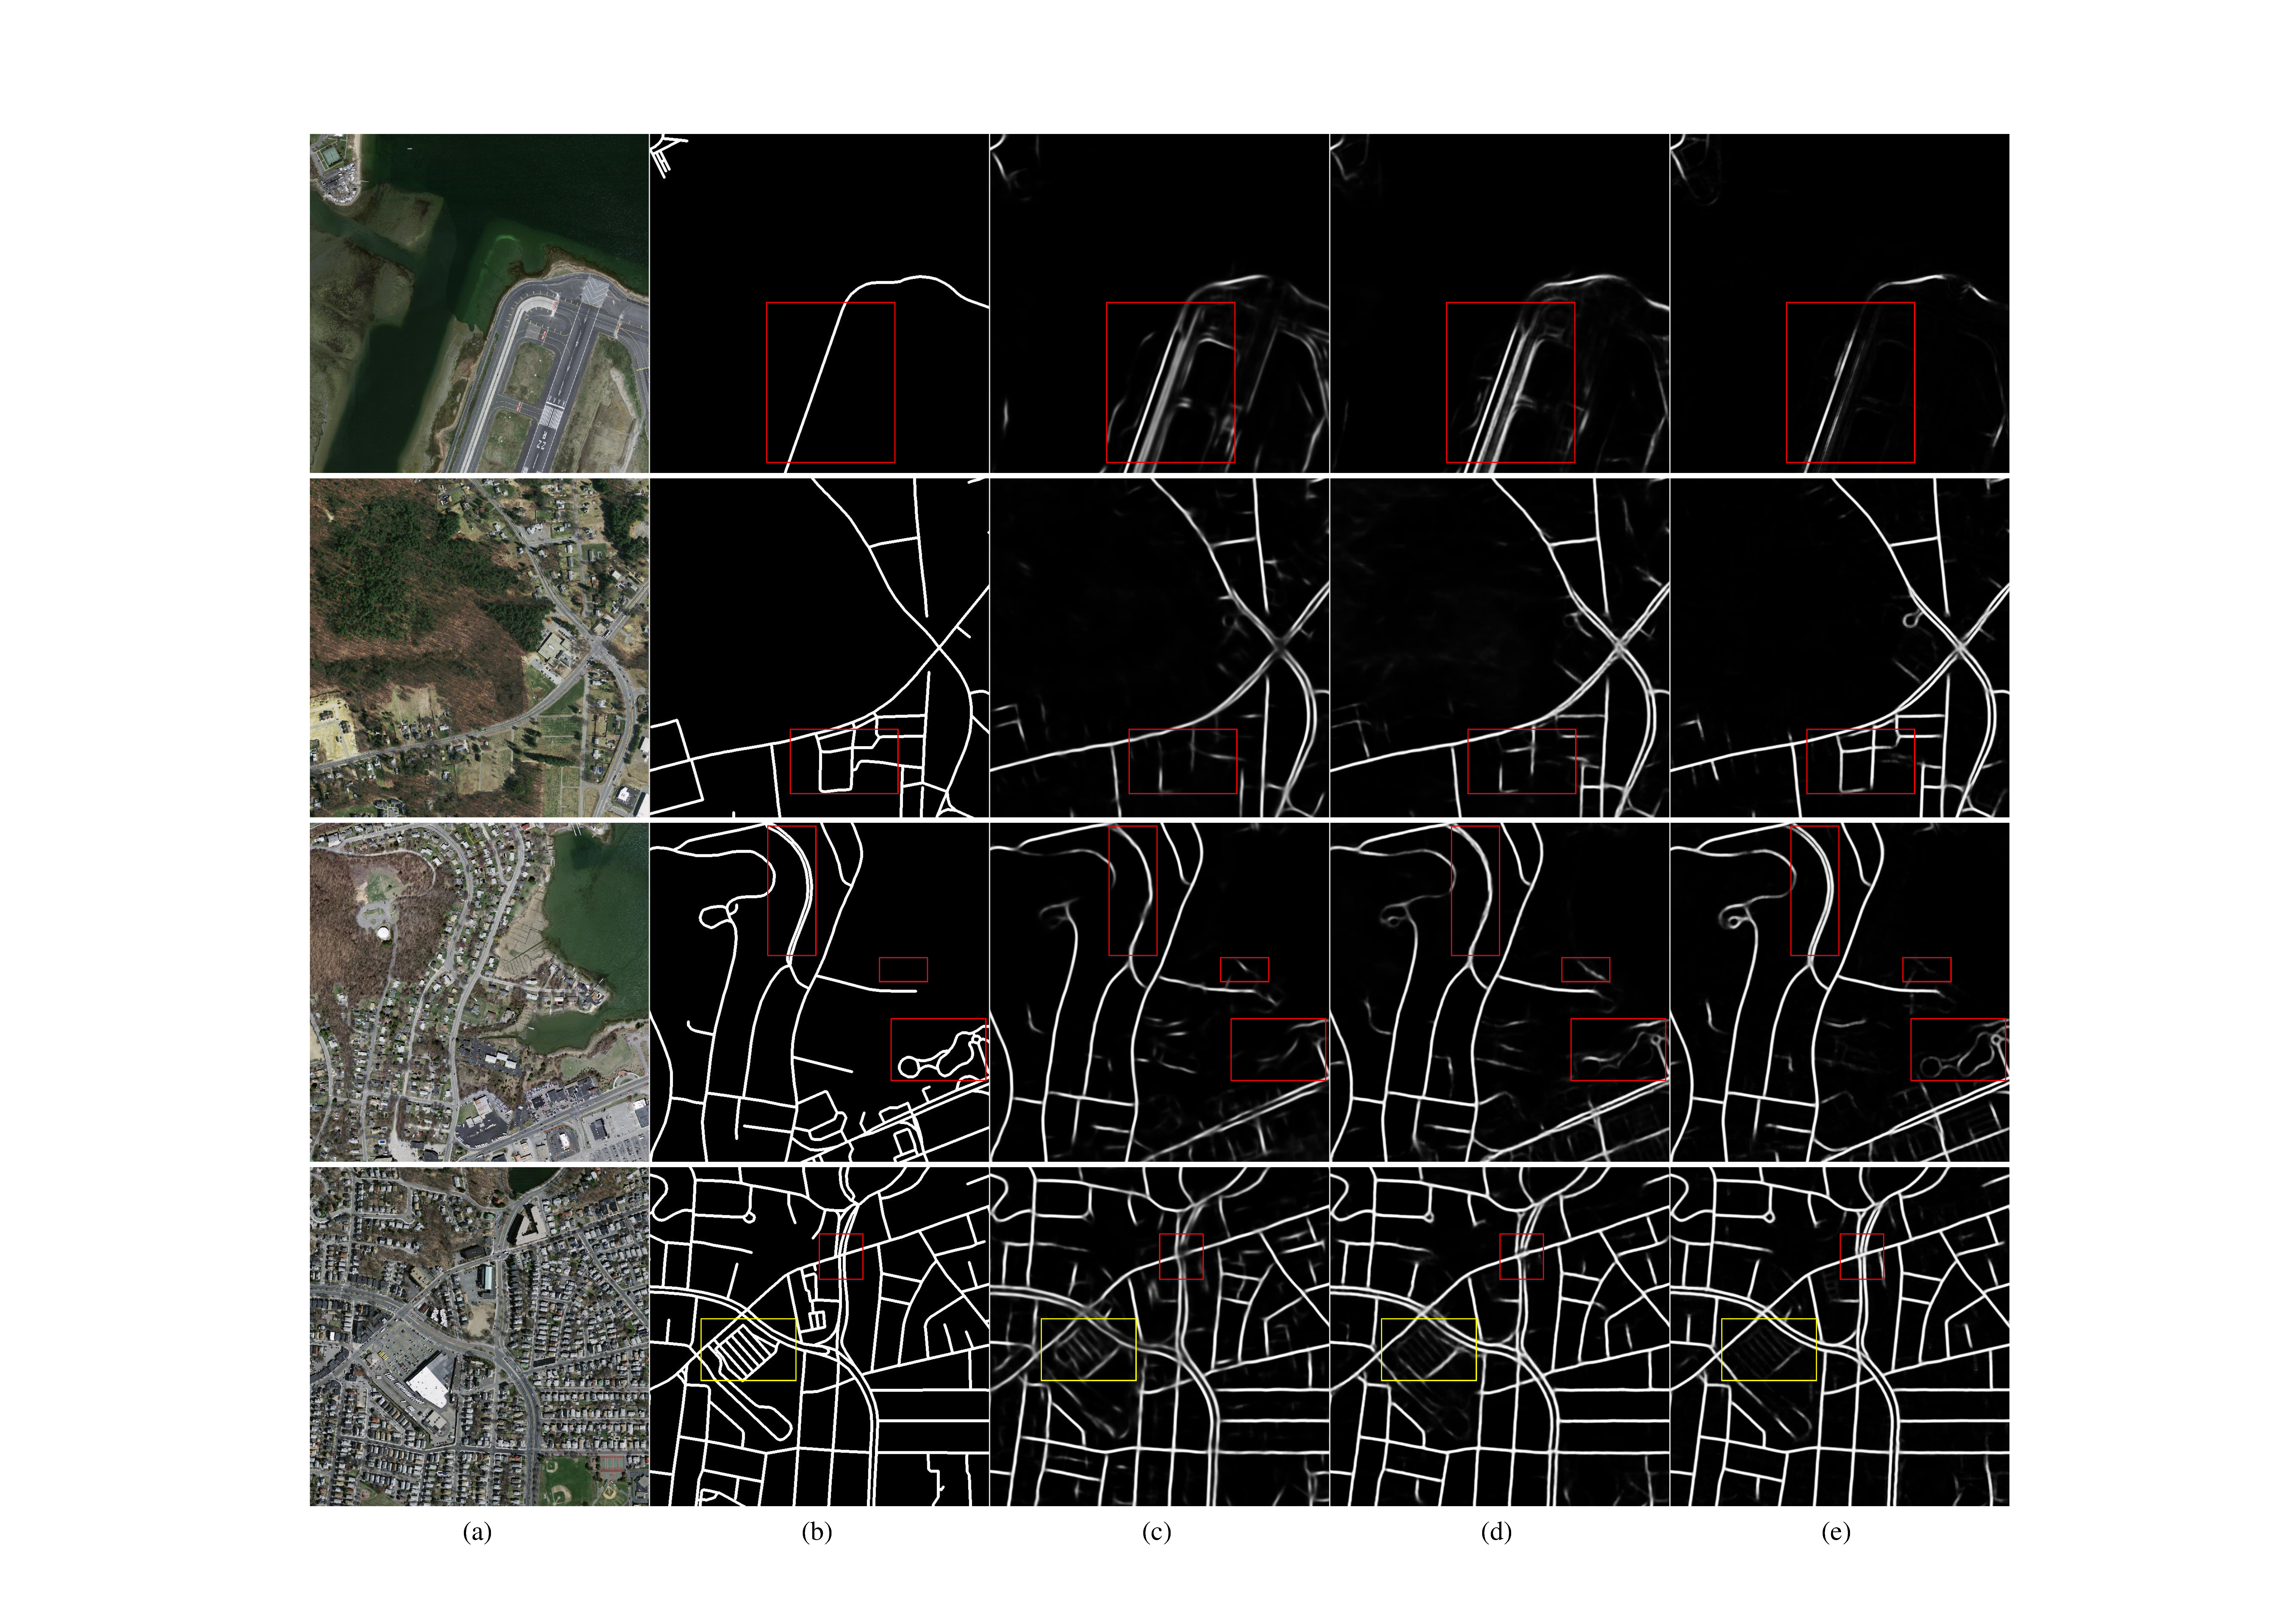
\includegraphics[width=1\textwidth]{imag_compare_2.pdf}
        \caption{马萨诸塞州道路数据集测试集的结果示例。(a) 输入图像;(b) 地面真相;(c) Saito等人~\cite{5};(d) U-Net ~\cite{24};(e) 本文方法结果。放大以查看更多详细信息。}
        \label{Fig:Result Comparison_0}
  \end{center}
\end{figure*}

图~\ref{Fig:Result Comparison_0}展示了Saito等人~\cite{5}的四个示例结果、U-Net~\cite{24}和我们所提出方法的结果。可以看出,与其他两种方法相比,我们的方法显示出更清晰的结果,并且噪声更小。特别是当有两条车道的道路时,我们的方法可以高置信度地分割每条车道,生成干净、清晰的两条车道道路,而其他方法可能会混淆车道,如图~\ref{Fig:Result Comparison_0}的第三行所示。同样,在相交区域,我们的方法也能产生更好的结果。

在分析具有复杂结构的对象时,上下文信息非常重要。我们的网络考虑了道路的上下文信息,因此可以将道路与类似对象(如建筑屋顶、机场跑道)区分开来。从图\ref{Fig:Result Comparison_0}的第一行可以看出,即使跑道具有与公路非常相似的特征,我们的方法也可以成功地从跑道分割出边路。除此之外,上下文信息还使其对遮挡具有鲁棒性。例如,第二行矩形上的部分道路被树木覆盖。Saito的方法和U-Net无法检测树下的道路,但我们的方法成功地标记了它们。故障案例显示在最后一行的黄色矩形中。我们的方法错过了停车场的道路。这主要是因为停车场的大多数道路都没有贴标签。因此,尽管这些道路与普通道路具有相同的特征,但考虑到上下文信息,我们的网络将其视为背景。

\section{结论}

在本文中,我们提出了从高分辨率遥感图像中提取道路的结果。该网络结合了残差学习和U-Net的优点。残差块内以及网络编码和解码路径之间的skip连接将促进了前向和后向计算中的信息传播。这种特性不仅便于训练,而且允许我们设计简单高效的神经网络。该网络的性能优于U-Net,仅需1/4的参数,以及其他两种基于深度学习的道路提取方法。

\appendix

% 书面翻译的参考文献
\bibliographystyle{unsrtnat}
\bibliography{ref/appendix}

% 书面翻译对应的原文索引
\begin{translation-index}
  \nocite{2017Road}
  \bibliographystyle{unsrtnat}
  \bibliography{ref/appendix}
\end{translation-index}

\end{translation}
